\documentclass[11pt, oneside]{book}
\usepackage[spanish]{babel}
\usepackage{fontspec}
\usepackage{amssymb}      % Necesario para los símbolos de flechas \blacktriangleleft y \blacktriangleright
\usepackage{tikz}
\usetikzlibrary{calc}
\usepackage{eso-pic}
\usepackage{graphicx}
\usepackage{float}
\usepackage{xcolor}
\usepackage{setspace}
\usepackage{titlesec}
\usepackage{caption}
\usepackage{array}
\usepackage{fancyhdr}     % Control exacto de encabezados y pies de página

% --- FUENTE PRINCIPAL: ARIAL (o Liberation Sans en Linux si no tienes Arial instalada) ---
\IfFontExistsTF{Arial}{
    \setmainfont{Arial}
}{
    \setmainfont{Liberation Sans} % Métricamente idéntica a Arial en Ubuntu
}

% --- FUENTE EXCLUSIVA PARA LOS NÚMEROS GIGANTES DE PORTADILLA (GOTHIC A1 EXTRA GRUESA) ---
\IfFontExistsTF{Gothic A1}{
    \newfontfamily\fuenteNumeroGigante{Gothic A1}[FakeBold=9.5]
}{
    \newfontfamily\fuenteNumeroGigante{Liberation Sans}[FakeBold=6]
}

% --- COLORES DEL DOCUMENTO Y DE LAS 10 PARTES ---
\definecolor{azulOscuro}{HTML}{12357A}
\definecolor{azulActivo}{HTML}{153B84}
\definecolor{grisBoton}{HTML}{99A1AE}
\definecolor{verdeAcento}{HTML}{7AE582}
\definecolor{grisTexto}{HTML}{333333}
\definecolor{grisMenu}{HTML}{666666}
\definecolor{fondoMenu}{HTML}{FFFFFF}

\definecolor{cPart1}{HTML}{123C73}
\definecolor{cPart2}{HTML}{3B1E6D}
\definecolor{cPart3}{HTML}{115793}
\definecolor{cPart4}{HTML}{2B6E23}
\definecolor{cPart5}{HTML}{B8860B}
\definecolor{cPart6}{HTML}{BA0C0C}
\definecolor{cPart7}{HTML}{2E77BB}
\definecolor{cPart8}{HTML}{9E3B6B}
\definecolor{cPart9}{HTML}{991B00}
\definecolor{cPart10}{HTML}{595959}

% --- GEOMETRÍA: MENÚ LATERAL (8.4 cm) + MÁRGENES DE 2.54 cm ---
\usepackage[
    a4paper,
    landscape,
    oneside,               % Evita que las páginas pares inviertan el margen izquierdo
    left=10.94cm,          % 8.4cm del menú lateral + 2.54cm de margen
    right=2.54cm,
    top=2.54cm,
    bottom=2.54cm
]{geometry}

% --- PIE DE PÁGINA: NÚMERO DE PÁGINA ABAJO A LA DERECHA (SIN ENCABEZADOS) ---
\pagestyle{fancy}
\fancyhf{}
\renewcommand{\headrulewidth}{0pt}
\renewcommand{\footrulewidth}{0pt}
\fancyfoot[R]{\fontsize{9}{11}\selectfont\color{grisMenu}\thepage}

\fancypagestyle{plain}{%
    \fancyhf{}%
    \renewcommand{\headrulewidth}{0pt}%
    \renewcommand{\footrulewidth}{0pt}%
    \fancyfoot[R]{\fontsize{9}{11}\selectfont\color{grisMenu}\thepage}%
}

% --- TIPOGRAFÍA Y ALINEACIÓN SOLICITADA ---
\onehalfspacing            % Interlineado 1.5
\raggedright               % Alineación izquierda (sin justificar)
\setlength{\parindent}{0pt}
\setlength{\parskip}{6pt}

% Capítulos Principales: Arial 18 pt, Negrita
\titleformat{\chapter}[display]
  {\fontsize{18}{22}\selectfont\bfseries\color{azulOscuro}}
  {}{0pt}{}
\titlespacing*{\chapter}{0pt}{-15pt}{12pt}

% Subsecciones (ej. 27.1): Arial 14 pt, Negrita
\titleformat{\section}
  {\fontsize{14}{17}\selectfont\bfseries\color{azulOscuro}}
  {\thesection}{0.6em}{}

% Sub-apartados internos: Arial 11 pt, Negrita
\titleformat{\subsection}
  {\fontsize{11}{14}\selectfont\bfseries\color{grisTexto}}
  {\thesubsection}{0.6em}{}

% Pie de figuras: Arial 8 pt
\DeclareCaptionFont{arial8}{\fontsize{8}{10}\selectfont\color{grisMenu}}
\captionsetup{
    font=arial8,
    justification=raggedright,
    singlelinecheck=false,
    labelsep=space
}

% --- HIPERVÍNCULOS ---
\usepackage[
    colorlinks=true,
    linkcolor=azulActivo,
    urlcolor=azulActivo,
    menucolor=grisBoton,
    bookmarks=true,
    bookmarksopen=true
]{hyperref}

% Variable que rastrea en qué parte (1 a 10) está el lector
\newcounter{parteActual}
\setcounter{parteActual}{0}

% Macro auxiliar: cuadros anchos (6.2cm + 0.95cm), altos (0.96cm) y letra grande (10.5pt)
\newcommand{\cajaBotonMenu}[3]{%
    \colorbox{#1}{%
        \parbox[c][0.96cm][c]{6.2cm}{\centering\fontsize{10.5}{12.5}\selectfont\bfseries\color{white}#2}%
    }\hspace{2pt}%
    \colorbox{#1}{%
        \parbox[c][0.96cm][c]{0.95cm}{\centering\fontsize{11.5}{13}\selectfont\bfseries\color{white}#3}%
    }%
}

% Macro para crear cada ítem del menú lateral
\newcommand{\itemMenuLateral}[2]{%
    \hyperlink{parte:#1}{%
        \ifnum\value{parteActual}=#1
            \cajaBotonMenu{azulActivo}{#2}{#1}%
        \else
            \cajaBotonMenu{grisBoton}{#2}{#1}%
        \fi
    }\\[4pt]
}

% --- DIBUJO AUTOMÁTICO DEL MENÚ IZQUIERDO EN CADA HOJA ---
\newcommand{\activarMenuLateral}{%
    \AddToShipoutPictureBG{%
        \begin{tikzpicture}[remember picture, overlay]
            % Fondo blanco limpio en la barra lateral ampliada
            \fill[fondoMenu] (current page.north west) rectangle ([xshift=8.3cm]current page.south west);

            % Logo superior izquierdo INFORMÁTICA®
            \node[anchor=north east, xshift=8.1cm, yshift=-1.8cm] at (current page.north west) {
                \fontsize{17}{20}\selectfont\bfseries\color{azulActivo}INFORMÁTICA\textsuperscript{\scriptsize®}
            };

            % Lista apilada de las 10 partes + flechas casi topadas al cuadro 10
            \node[anchor=north west, xshift=0.35cm, yshift=-3.8cm] at (current page.north west) {
                \begin{minipage}{8.6cm}
                    \itemMenuLateral{1}{Orígenes: Del Cálculo Manual a la Máquina}
                    \itemMenuLateral{2}{La Era Electrónica}
                    \itemMenuLateral{3}{Fundamentos de la Informática y el Hardware}
                    \itemMenuLateral{4}{Sistemas Operativos}
                    \itemMenuLateral{5}{Bases de Datos}
                    \itemMenuLateral{6}{Lenguajes de Programación}
                    \itemMenuLateral{7}{Redes, Internet y Ciberseguridad}
                    \itemMenuLateral{8}{La Era Moderna}
                    \itemMenuLateral{9}{Tendencias a Futuro}
                    \itemMenuLateral{10}{Anexos y Glosarios}
                    
                    \vspace{4pt}
                    \parbox{7.65cm}{\centering
                        {\hypersetup{menucolor=grisBoton, linkcolor=grisBoton}%
                        \fontsize{15}{17}\selectfont
                        \Acrobatmenu{PrevPage}{\textcolor{grisBoton}{$\blacktriangleleft$}} \hspace{0.5cm}%
                        \Acrobatmenu{NextPage}{\textcolor{grisBoton}{$\blacktriangleright$}}}
                    }
                \end{minipage}
            };
        \end{tikzpicture}%
    }%
}

% Macro para iniciar cada una de las 10 partes
\newcommand{\iniciarParte}[3]{%
    \clearpage
    \thispagestyle{plain}   % Muestra el número de página abajo a la derecha desde la pág. 3
    \setcounter{parteActual}{#1}
    \hypertarget{parte:#1}{}
    \pdfbookmark[0]{Parte #1: #2}{parte:#1}

    % Dibuja el número gigante (#1.) DE FONDO (BG) completo y sin cortarse
    \AddToShipoutPictureBG*{%
        \begin{tikzpicture}[remember picture, overlay]
            \node[
                anchor=north east,
                inner sep=0pt,
                outer sep=0pt,
                xshift=-0.35cm,
                yshift=-0.35cm
            ] at (current page.north east) {
          \scalebox{24}{\fuenteNumeroGigante\color{azulActivo!38}#1\kern-0.01em\raisebox{-0.013em}{\scalebox{0.75}{.}}}};
         \end{tikzpicture}%
    }

    % Título proporcionado (28pt) que queda limpio por encima del número de fondo
    \vspace*{2.2cm}
    \begin{minipage}[t]{0.92\textwidth}
        \raggedright
        \fontsize{28}{34}\selectfont\bfseries\color{azulActivo}
        \MakeUppercase{#2}
    \end{minipage}

    \clearpage
    % Carga el contenido de esa parte
    \input{#3}
}

\begin{document}

% =========================================================================
% PÁGINA 1: IMAGEN A PÁGINA COMPLETA (SIN MÁRGENES NI MENÚ)
% =========================================================================
\thispagestyle{empty}
\AddToShipoutPictureBG*{%
    \AtPageLowerLeft{%
        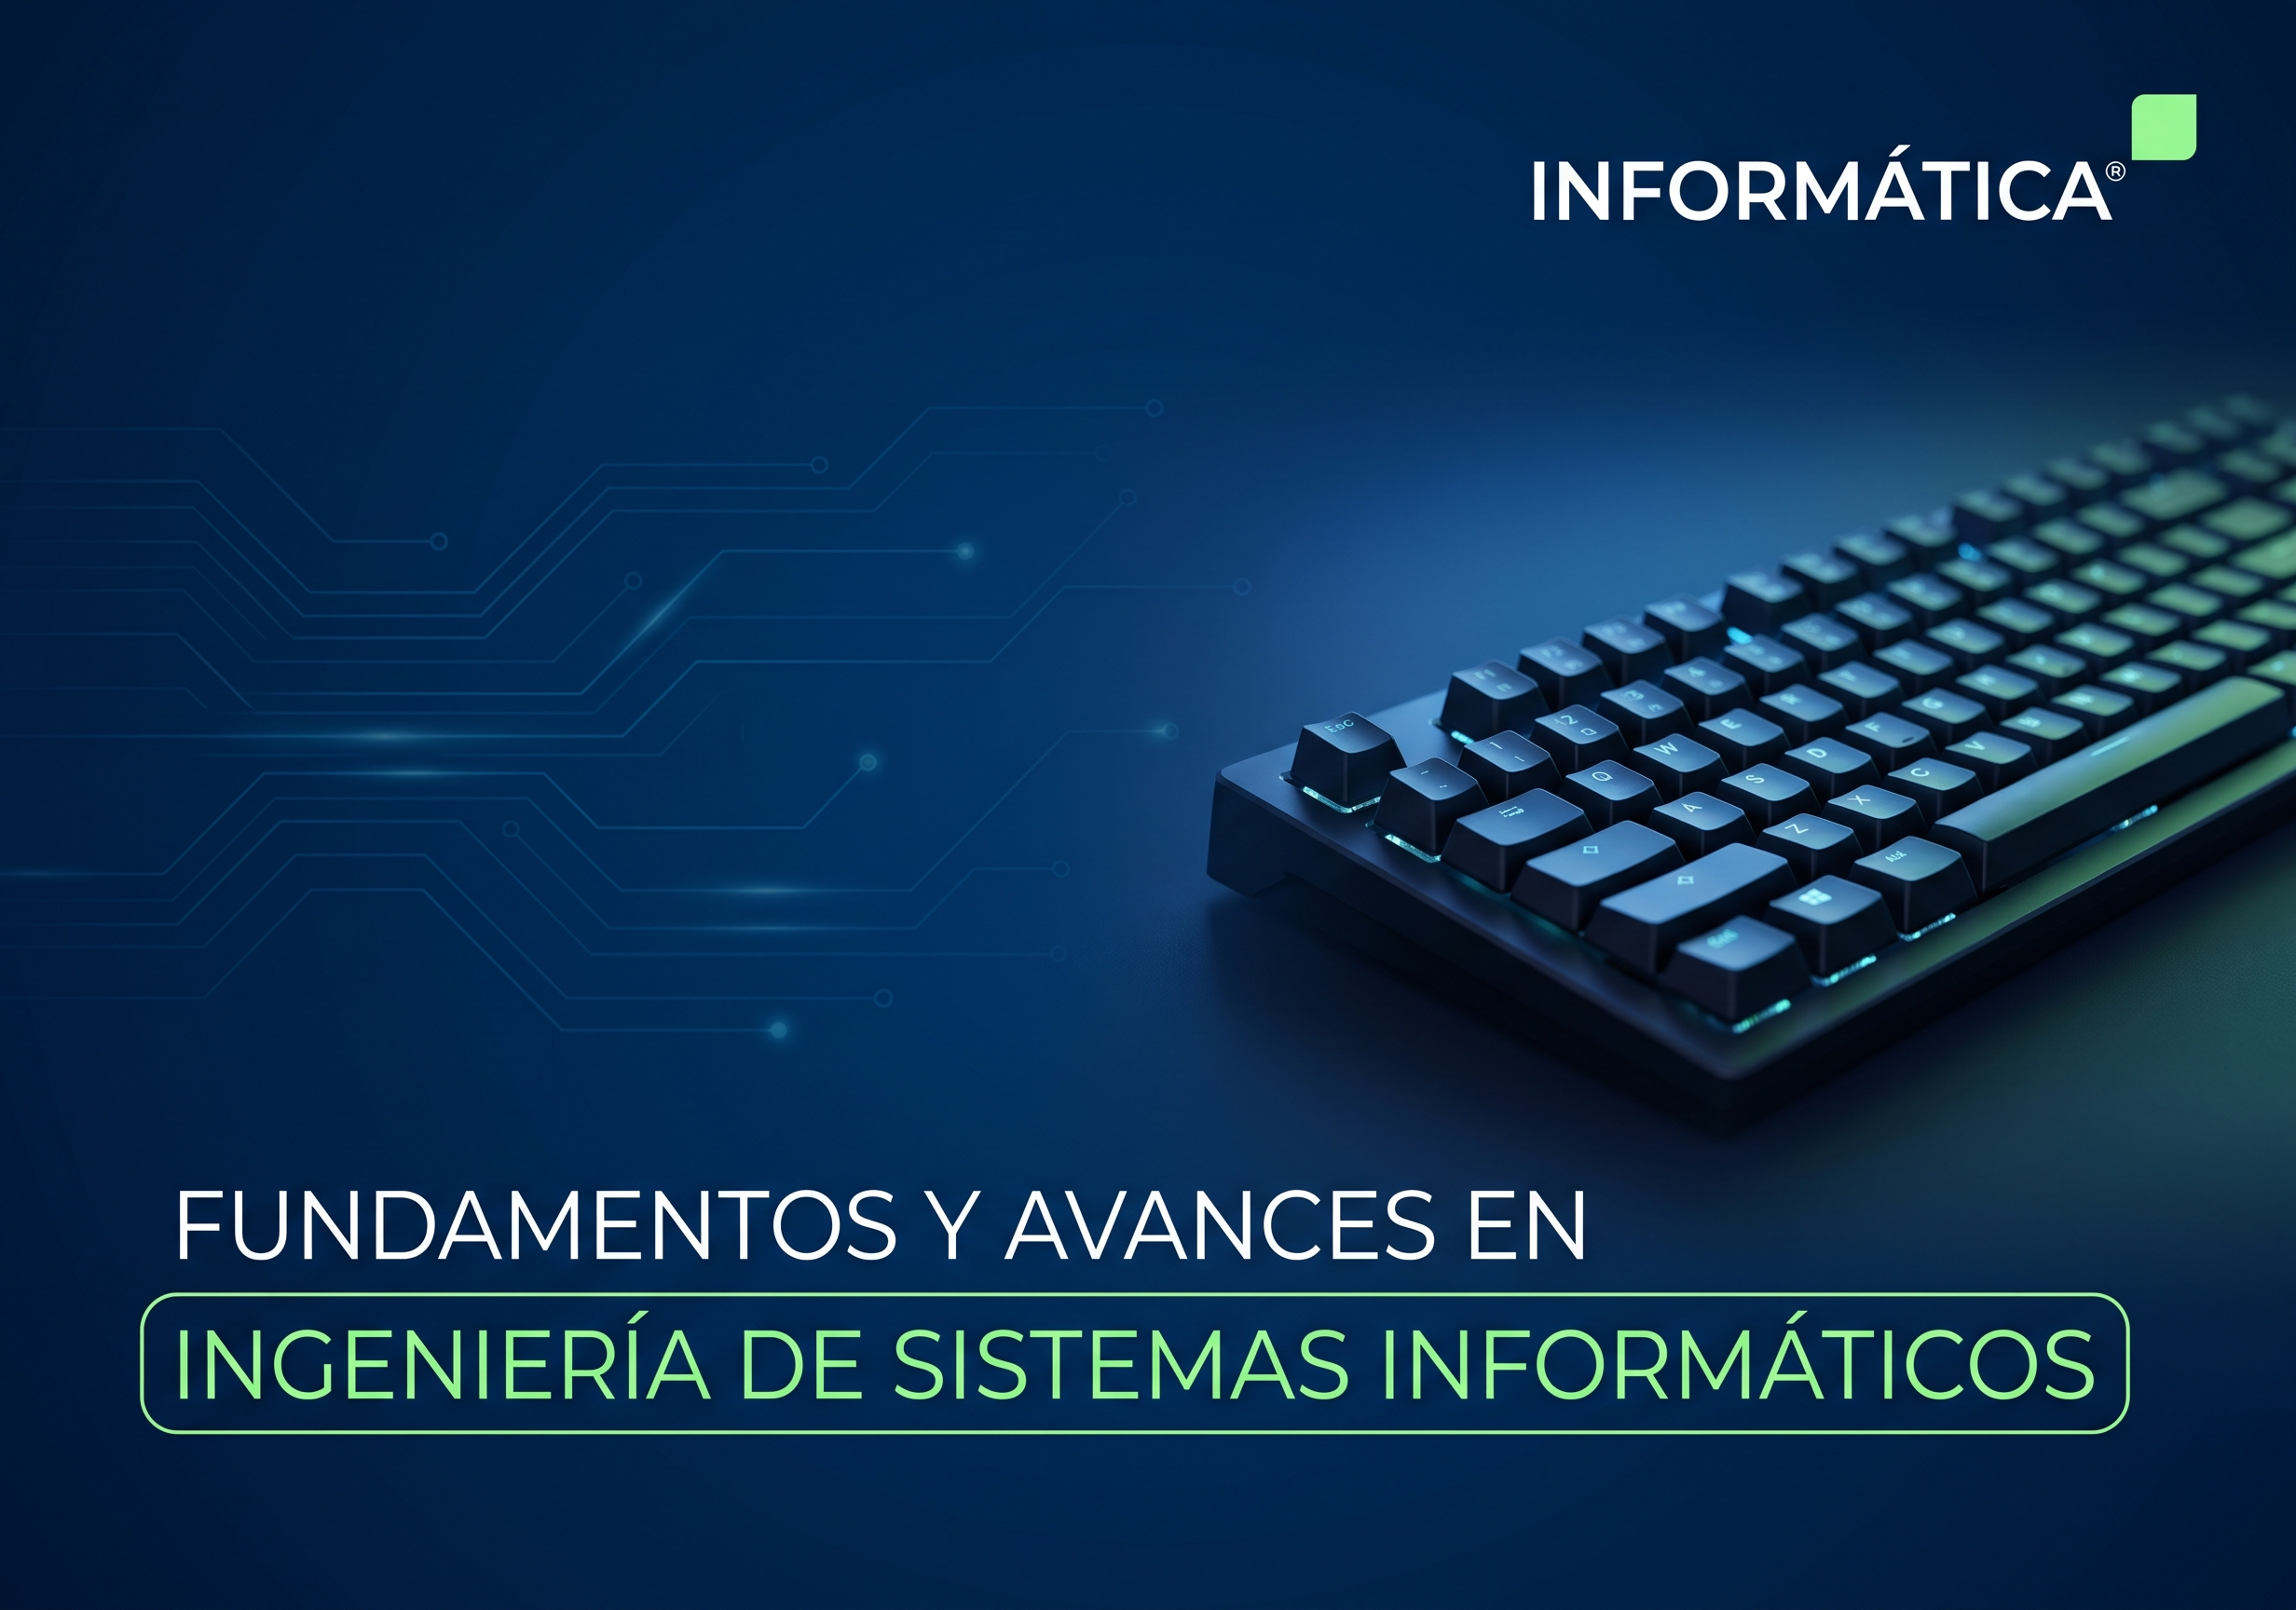
\includegraphics[width=\paperwidth, height=\paperheight]{imagenes/portada.jpg}%
    }%
}
\null
\clearpage

% =========================================================================
% PÁGINA 2: ÍNDICE GENERAL DE 2 COLUMNAS CON COLORES + INTRODUCCIÓN AZUL
% =========================================================================
\newgeometry{left=1.2cm, right=1.2cm, top=2cm, bottom=1.2cm}
\thispagestyle{empty}

% Macro para dibujar cada bloque de parte exactamente como tu diseño
\newcommand{\bloqueParte}[4]{%
    \hyperlink{parte:#1}{%
        \begin{minipage}[t]{\linewidth}
            \colorbox{#2}{%
                \parbox{\dimexpr\linewidth-2\fboxsep\relax}{%
                    \color{white}\fontsize{8.5}{10}\selectfont\bfseries
                    \makebox[0.55cm][c]{#1}%
                    \hspace{1pt}\rule[-2pt]{1pt}{10pt}\hspace{5pt}%
                    #3%
                }%
            }\\[6pt]
            {\fontsize{8}{10.5}\selectfont\color{grisTexto}\raggedright #4}%
        \end{minipage}%
    }\\[24pt]
}

% --- COLUMNA 1: PARTES 1 A 5 ---
\begin{minipage}[t]{0.315\textwidth}
    \vspace{0.8cm}
    \bloqueParte{1}{cPart1}{Orígenes: Del Cálculo Manual a la Máquina}{Evolución histórica desde los primeros instrumentos numéricos hasta las máquinas mecánicas y electromecánicas.}
    \bloqueParte{2}{cPart2}{La Era Electrónica}{Nacimiento de los primeros ordenadores electrónicos, la definición de la arquitectura Von Neumann y la invención del microprocesador.}
    \bloqueParte{3}{cPart3}{Fundamentos de la Informática y Hardware}{Principios de lógica digital, circuitos y el funcionamiento interno de la CPU, memorias y periféricos.}
    \bloqueParte{4}{cPart4}{Sistemas Operativos: Gestión de Recursos}{Evolución del software base, administración de procesos, memoria, almacenamiento y virtualización en entornos modernos.}
    \bloqueParte{5}{cPart5}{Bases de Datos y Gestión de Información}{Modelos de almacenamiento desde archivos planos y sistemas relacionales hasta arquitecturas NoSQL, Big Data y bases vectoriales.}
\end{minipage}
\hfill
% --- COLUMNA 2: PARTES 6 A 10 ---
\begin{minipage}[t]{0.315\textwidth}
    \vspace{0.8cm}
    \bloqueParte{6}{cPart6}{Lenguajes de Programación y Software}{Historia del código, desarrollo de paradigmas de programación e ingeniería de software moderna con prácticas DevOps.}
    \bloqueParte{7}{cPart7}{Redes, Internet y Ciberseguridad}{Origen de las comunicaciones, arquitectura TCP/IP, evolución Web, modelos Cloud y fundamentos de ciberdefensa.}
    \bloqueParte{8}{cPart8}{La Era Moderna e Inteligencia Artificial}{Evolución de la IA, aprendizaje profundo, modelos generativos (LLM), agentes autónomos y conceptos de computación cuántica.}
    \bloqueParte{9}{cPart9}{Tendencias a Futuro y Prospectiva}{Análisis del impacto socioeconómico, ética algorítmica, interacción humano-computadora avanzada y horizontes hacia la AGI.}
    \bloqueParte{10}{cPart10}{Anexos y Glosario}{Recopilación de líneas temporales, biografías clave, tablas comparativas de lenguajes, glosario técnico y bibliografía.}
\end{minipage}
\hfill
% --- COLUMNA 3: LOGO DERECHO + TEXTO INTRODUCTORIO EN AZUL (INTERLINEADO 2) ---
\begin{minipage}[t]{0.31\textwidth}
    \vspace{0pt}
    {\raggedleft \fontsize{15}{17}\selectfont\bfseries\color{cPart1} INFORMÁTICA\textsuperscript{\scriptsize®} \par}
    \vspace{0.6cm}

    {\doublespacing\fontsize{9}{11}\selectfont\color{cPart3}\raggedright
    Cada estudiante y profesional de la informática recorre un camino único, desde la comprensión de la lógica binaria fundamental hasta el diseño de sistemas distribuidos y la gestión de inteligencia artificial.

    \vspace{0.4cm}
    Esta obra reúne en un solo lugar todo el núcleo de conocimientos de la carrera de Ingeniería en Informática. El texto analiza en profundidad desde los orígenes del cálculo y la arquitectura física del hardware, hasta la abstracción de los sistemas operativos, el modelado de datos, la ingeniería de software, las redes globales y las fronteras de la IA moderna.

    \vspace{0.4cm}
    Además de servir como compendio académico, este libro proporciona el marco conceptual y práctico para estructurar, conectar y aplicar cada materia vista en las aulas en entornos reales.

    \vspace{0.4cm}
    Está diseñado para acompañar tanto al estudiante en su formación como al graduado y docente en su ejercicio profesional, ofreciendo una visión integral, analítica y actualizada del ecosistema tecnológico actual.\par}
\end{minipage}

\restoregeometry
\clearpage

% =========================================================================
% PÁGINA 3 EN ADELANTE: ACTIVA EL MENÚ LATERAL FIJO Y LAS 10 PARTES
% =========================================================================
\activarMenuLateral

\iniciarParte{1}{Orígenes del Cálculo Manual a la Máquina}{partes/parte01}
\iniciarParte{2}{La Era Electrónica: Nacimiento de la Computadora Moderna}{partes/parte02}
\iniciarParte{3}{Fundamentos de la Informática y el Hardware}{partes/parte03}
\iniciarParte{4}{Sistemas Operativos: La Gestión del Recurso Computacional}{partes/parte04}
\iniciarParte{5}{Bases de Datos y Gestión de la Información}{partes/parte05}
\iniciarParte{6}{Lenguajes de Programación y Desarrollo de Software}{partes/parte06}
\iniciarParte{7}{Redes, Internet y Ciberseguridad}{partes/parte07}
\iniciarParte{8}{La Era Moderna: Inteligencia Artificial y Estado del Arte (Hasta 2026)}{partes/parte08}
\iniciarParte{9}{Tendencias a Futuro y Prospectiva Tecnológica}{partes/parte09}
\iniciarParte{10}{Anexos y Glosario}{partes/parte10}

\end{document}